\documentclass[12pt, a4paper]{article}
\usepackage[a4paper,top=1.5cm, bottom=1.5cm, left=2cm, right=2cm]{geometry}
\usepackage{graphicx} % Required for inserting images
%%% Работа с русским языком
\usepackage{cmap}					% поиск в PDF
\usepackage{mathtext} 				% русские буквы в фомулах
\usepackage[T2A]{fontenc}			% кодировка
\usepackage[utf8]{inputenc}			% кодировка исходного текста
\usepackage[english,russian]{babel}	% локализация и переносы
\usepackage{float}
\usepackage{subcaption}
\usepackage{wrapfig}
\usepackage{tabularx}
\usepackage{multirow}

\usepackage[unicode, colorlinks=true, urlcolor=blue]{hyperref}
\usepackage[rgb]{xcolor}
\hypersetup{
colorlinks=true,urlcolor=blue
}
%%% Дополнительная работа с математикой
\usepackage{amsmath,amsfonts,amssymb,amsthm,mathtools} % AMS
\usepackage{icomma} % "Умная" запятая: $0,2$ --- число, $0, 2$ --- перечисление
%% Номера формул
\mathtoolsset{showonlyrefs=true} % Показывать номера только у тех формул, на которые есть \eqref{} в тексте.
%% Шрифты
\usepackage{euscript}	 % Шрифт Евклид
\usepackage{mathrsfs} % Красивый матшрифт
%% Свои команды
\DeclareMathOperator{\sgn}{\mathop{sgn}}
%% Перенос знаков в формулах (по Львовскому)
\newcommand*{\hm}[1]{#1\nobreak\discretionary{}
{\hbox{$\mathsurround=0pt #1$}}{}}


\usepackage{indentfirst}
\usepackage{amsmath,amssymb}
\usepackage[italicdiff]{physics}
\graphicspath{{images/}}
\DeclareGraphicsExtensions{.pdf,.png,.jpg}
\usepackage{enumitem}
\usepackage{caption}
\usepackage{array}
\usepackage{ragged2e}

\usepackage{tikz}
\usetikzlibrary{arrows,decorations.markings,calc}
\usetikzlibrary{arrows.meta, calc, patterns}







\begin{document}



\include{titlepage}
\begin{titlepage}
\thispagestyle{empty}

\begin{center}
\small
Министерство науки и высшего образования Российской Федерации\\[2mm]
\textbf{ФЕДЕРАЛЬНОЕ ГОСУДАРСТВЕННОЕ АВТОНОМНОЕ
ОБРАЗОВАТЕЛЬНОЕ УЧРЕЖДЕНИЕ ВЫСШЕГО ОБРАЗОВАНИЯ}\\[1mm]
«МОСКОВСКИЙ ФИЗИКО-ТЕХНИЧЕСКИЙ ИНСТИТУТ\\
(НАЦИОНАЛЬНЫЙ ИССЛЕДОВАТЕЛЬСКИЙ УНИВЕРСИТЕТ)»\\
(МФТИ, Физтех)
\end{center}

\vspace{18mm}

\begin{center}
\large \textbf{КАФЕДРА КВАНТОВОЙ ЭЛЕКТРОНИКИ}\\[10mm]
\Large \textbf{ОТЧЁТ}\\[2mm]
\large \textbf{ПО ЛАБОРАТОРНОЙ РАБОТЕ}\\[14mm]
\Large \textbf{ОПТИКА ЛАЗЕРНЫХ ПУЧКОВ}
\end{center}

\vfill

% Блоки с подписями слева, линии и пояснения справа
\noindent
\begin{tabular}{@{}p{0.44\linewidth}p{0.52\linewidth}@{}}
\textit{Работу выполнили:} & Вакорина Анастасия,

Винокуров Владислав,

Выгнанчук Валерия,

Ескина Ольга,

Рагозина Елизавета,

Струков Олег,

Группа Б04-404 \\[8mm]

\textit{Работу принял, оценка:} & \\[3mm]
 \\
\end{tabular}


\vspace{12mm}

\begin{center}
\small Долгопрудный, \the\year{}~г.
\end{center}

\end{titlepage}










\newpage

\section*{Теоретическая часть}

\subsection*{1. Гауссовы оптические системы и лучевые матрицы}
В параксиальном приближении любую оптическую систему, состоящую из линз, зеркал и участков однородной среды, можно описать с помощью лучевой матрицы (матрицы ABCD) размером $2 \times 2$. Геометрический луч в плоскости $z = \text{const}$ характеризуется расстоянием $x$ от оптической оси и углом наклона $\alpha$ к ней.

\begin{figure}[h]
\centering
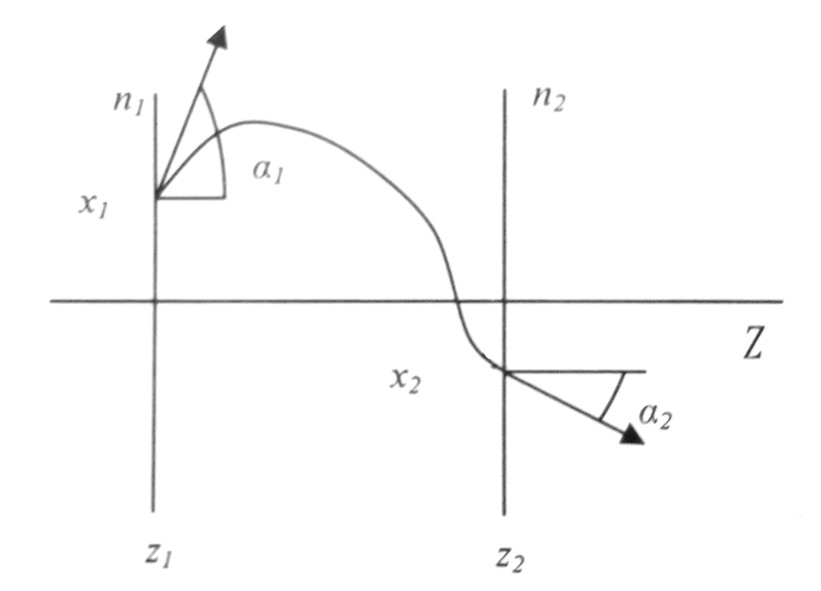
\includegraphics[width=0.4\textwidth]{1.jpg}
\caption{Прохождение луча через гауссову оптическую систему}
\label{fig:ray_matrix}
\end{figure}

На выходе системы координаты луча связаны с входными линейными соотношениями:
\begin{equation}
    \begin{pmatrix} x_2 \\ \alpha_2 \end{pmatrix} = 
    \begin{pmatrix} A & B \\ C & D \end{pmatrix} 
    \begin{pmatrix} x_1 \\ \alpha_1 \end{pmatrix} = M \begin{pmatrix} x_1 \\ \alpha_1 \end{pmatrix},
\end{equation}
где $M$ --- лучевая матрица системы. Для последовательно расположенных элементов полная матрица равна произведению матриц отдельных элементов в порядке, обратном ходу луча: $M_{\text{общ}} = M_n \cdot \ldots \cdot M_1$. Определитель матрицы $AD - BC = n_1 / n_2$, где $n_1$ и $n_2$ --- показатели преломления сред на входе и выходе (в воздухе $n_1 = n_2 = 1$, поэтому $AD - BC = 1$).

\begin{table}[h]
\centering
\caption{Лучевые матрицы простейших оптических элементов}
\label{tab:matrices}
\begin{tabular}{|c|l|c|}
\hline
№ & Оптический элемент & Лучевая матрица $M$ \\
\hline
1 & Среда с показателем преломления $n$, длина $d$ & $\begin{pmatrix} 1 & d/n \\ 0 & 1 \end{pmatrix}$ \\
\hline
2 & Тонкая линза с фокусным расстоянием $f$ & $\begin{pmatrix} 1 & 0 \\ -1/f & 1 \end{pmatrix}$ \\
\hline
3 & Сферическое зеркало радиуса кривизны $R$ & $\begin{pmatrix} 1 & 0 \\ -2/R & 1 \end{pmatrix}$ \\
\hline
\end{tabular}
\end{table}

\subsection*{2. Оптика гауссовых пучков и закон ABCD}
Для описания распространения волновых пучков света вводится комплексный параметр гауссова пучка $q$, связанный с радиусом кривизны фазового фронта $R(z)$ и характерным поперечным размером пучка $\omega(z)$ (на уровне спада интенсивности в $e^2$ раз):
\begin{equation}
    \frac{1}{q(z)} = \frac{1}{R(z)} - i \frac{\lambda}{\pi \omega^2(z)},
\end{equation}
где $\lambda$ --- длина волны излучения. 

Главное свойство гауссова пучка: при прохождении через любую гауссову оптическую систему он остаётся гауссовым, а его параметр $q$ преобразуется по \textbf{закону ABCD}:
\begin{equation}
    q_2 = \frac{A q_1 + B}{C q_1 + D},
\end{equation}
где $A, B, C, D$ --- элементы лучевой матрицы системы. 

Для свободного пространства длиной $z$ при условии плоского фазового фронта в перетяжке ($z=0$, $R=\infty$, $q_0 = i\pi\omega_0^2/\lambda$) зависимости имеют вид:
\begin{equation}
    \omega^2(z) = \omega_0^2 \left[ 1 + \left(\frac{\lambda z}{\pi \omega_0^2}\right)^2 \right], \qquad
    R(z) = z \left[ 1 + \left(\frac{\pi \omega_0^2}{\lambda z}\right)^2 \right].
\end{equation}
Угол расходимости пучка в дальней зоне определяется как $\theta = \lambda / (\pi \omega_0)$.

\begin{figure}[h]
\centering
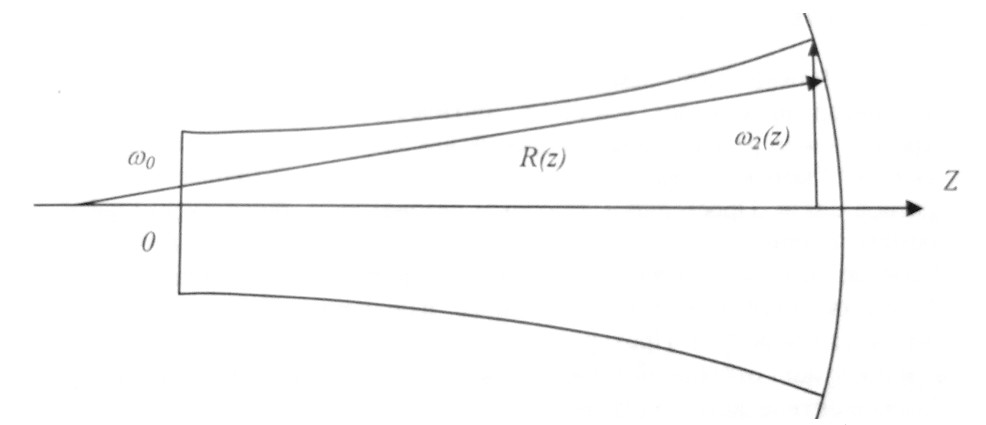
\includegraphics[width=0.6\textwidth]{2.jpg}
\caption{Изменение размера пучка $\omega(z)$ и радиуса кривизны $R(z)$ вдоль оси распространения}
\label{fig:gaussian_beam}
\end{figure}

\subsection*{3. Устойчивость лазерных резонаторов}
Резонатор считается устойчивым, если гауссов пучок может существовать в нём, неограниченно повторяя свою поперечную структуру при обходах. Условие устойчивости определяется через элементы матрицы полного обхода резонатора:
\begin{equation}
    -1 < \frac{A + D}{2} < 1.
\end{equation}
Для классического двухзеркального резонатора длиной $L$ с зеркалами радиусов кривизны $R_1$ и $R_2$ это условие эквивалентно $0 \le g_1 g_2 \le 1$, где $g_i = 1 - L/R_i$. 

\begin{figure}[h]
\centering
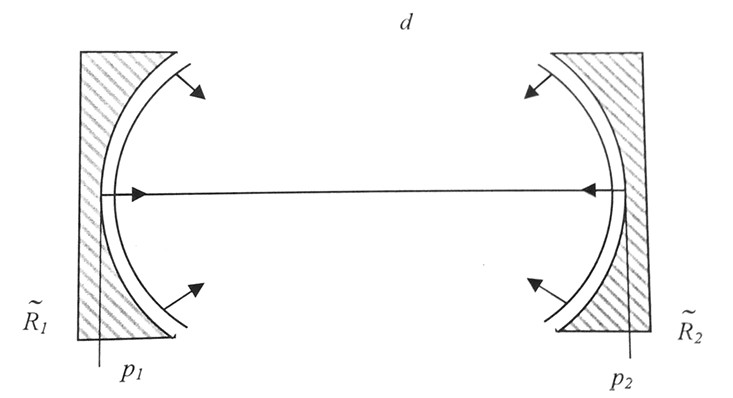
\includegraphics[width=0.5\textwidth]{3.jpg}
\caption{Схема двухзеркального резонатора и резонатора с внутрирезонаторной линзой}
\label{fig:resonator}
\end{figure}

Резонатор со сложной внутрирезонаторной оптикой (например, с линзой) удобно сводить к эквивалентному двухзеркальному резонатору с эффективными длинами плеч и эффективными радиусами кривизны зеркал. Параметр пучка $q$ внутри устойчивого резонатора находится из условия самосогласования $q = (Aq + B)/(Cq + D)$.

Наличие ограничивающей апертуры радиусом $R_a$ определяет модовый состав излучения. Если $\omega_0 \sim (0,5 \div 1) R_a$, в генерации участвует только мода нулевого порядка TEM$_{00}$ (одномодовый режим), так как моды высших порядков испытывают большие дифракционные потери.

\subsection*{4. Метод измерения поперечного размера пучка}
Экспериментальное определение размера пучка $\omega$ проводится путём сканирования поперечного сечения пучка фотоприёмником, перемещаемым микрометрическим винтом. Для гауссова пучка нулевого порядка распределение интенсивности описывается выражением:
\begin{equation}
    I(x) = I_0 \exp\left(-\frac{2x^2}{\omega^2}\right).
\end{equation}
Логарифмируя это выражение, получаем линейную зависимость:
\begin{equation}
    \ln I(x) = \ln I_0 - \frac{2}{\omega^2} x^2.
\end{equation}
Построение экспериментальной зависимости $\ln I(x)$ от $x^2$ и аппроксимация её прямой линией позволяют определить характерную полуширину пучка $\omega$ из углового коэффициента $k$ полученной прямой:
\begin{equation}
    \omega = \sqrt{-\frac{2}{k}}.
\end{equation}
Этот же метод, в сочетании с законом ABCD, применяется для экспериментального определения фокусного расстояния линзы по изменению параметра $\omega$ до и после неё.

% \begin{figure}[h]
% \centering
% \includegraphics[width=0.6\textwidth]{fig4_measurement.png}
% \caption{Схема сканирования пучка и линеаризация зависимости интенсивности}
% \label{fig:measurement}
% \end{figure}









\section*{Ход работы}

\subsection*{Экспериментальная установка и суть метода}

В работе используется схема сканирования поперечного профиля пучка He-Ne лазера ($\lambda = 0{,}6328$ мкм). Фотоприёмник со щелью на микрометрической подвижке последовательно перемещается вдоль оси $x$, «срезая» пучок, а вольтметр регистрирует напряжение $U(x)$, пропорциональное интенсивности. При необходимости в оптический путь вводится линза с фокусным расстоянием $f$. Полученная зависимость $U(x)$ позволяет восстановить профиль пучка и определить его характерный размер $\omega$.
\begin{figure}[h]
\centering
\begin{tikzpicture}[scale=0.9, >=Stealth, font=\small]
    % Лазер
    \draw[thick, fill=gray!20] (0, -0.8) rectangle (2.5, 0.8);
    \node at (1.25, 0) {He-Ne лазер};
    \node[above] at (1.25, 0.8) {$\lambda = 0{,}6328$ мкм};
    
    % Пучок (конус)
    \fill[red!15] (2.5, 0) -- (9.5, 1.0) -- (9.5, -1.0) -- cycle;
    \draw[thick, red] (2.5, 0) -- (9.5, 0); 
    
    % Линза (пунктиром, так как она добавляется на втором этапе)
    \draw[thick, blue, double, double distance=2pt] (5.5, -2) -- (5.5, 2);
    \node[above, blue] at (5.5, 2) {Линза ($f$)};
    
    % Фотоприёмник
    \draw[thick, fill=gray!50] (9.5, -1.2) rectangle (10, 1.2);
    \node[right, align=left] at (10, 0) {Фотоприёмник\\с щелью};
    
    % Микрометрическая подвижка
    \draw[thick] (9.75, -1.2) -- (9.75, -2);
    \draw[thick, ->] (11.5, -2) -- (10.2, -2);
    \node[below] at (11.5, -2) {Микрометрический винт ($x$)};
    
    % Вольтметр
    \draw[thick] (10, 1.2) -- (10, 2.8) -- (12, 2.8);
    \draw[thick] (12, 2.3) circle (0.5);
    \node at (12, 2.3) {V};
    \node[above] at (12, 3.3) {Вольтметр};
    
    % Расстояния
    \draw[<->] (2.5, -2.8) -- (9.5, -2.8);
    \node at (6, -3.1) {$z$ };   %(или $d_1 + d_2$)
    
    % Оптическая ось
    \draw[dashed, ->] (2.5, 0) -- (13, 0) node[right] {$z$};
\end{tikzpicture}
\caption{Схема экспериментальной установки для измерения поперечного профиля гауссова пучка}
\label{fig:setup}
\end{figure}


\subsection*{Измерение профиля пучка без линзы}

Для определения параметров гауссова пучка, выходящего из He-Ne лазера, были проведены измерения поперечного распределения интенсивности излучения на двух различных расстояниях от выходного окна лазера: $z_A = 49,2$ см и $z_B = 79,7$ см. 

Фотоприёмник, установленный на микрометрической подвижке, последовательно сканировал пучок в поперечном направлении, а регистрируемое напряжение $U$, пропорциональное интенсивности света, записывалось как функция координаты $x$. Обе снятые зависимости имеют характерный вид гауссова распределения, что подтверждает одномодовый режим генерации лазера (мода TEM$_{00}$).

\subsection*{Обработка результатов: определение поперечного размера пучка $\omega$}

Для каждой из снятых зависимостей была проведена линеаризация данных. Поскольку центр пучка в эксперименте был смещён относительно нулевой отметки микрометрического винта, координата была переопределена как $x' = x - x_c$, где $x_c$ --- координата максимума интенсивности.

Зависимость $\ln(U)$ от $(x')^2$ аппроксимировалась прямой линией вида:
\begin{equation}
    \ln(U) = \ln U_0 - \frac{2}{\omega^2} (x')^2.
\end{equation}

По угловому коэффициенту $k$ полученной прямой характерный поперечный размер пучка вычислялся по формуле $\omega = \sqrt{-2/k}$. Результаты представлены на рис.~\ref{fig:linearization} и в таблице~\ref{tab:omega_results}:

\begin{table}[h]
\centering
\caption{Результаты определения размера пучка $\omega$ методом линеаризации}
\label{tab:omega_results}
\begin{tabular}{|c|c|c|c|}
\hline
Расстояние $z$, см & $x_c$, мм & Угловой коэфф. $k$, мм$^{-2}$ & $\omega$, мм \\
\hline
49,2 & 0,792 & $-24,6$ & $0,285 \pm 0,003$ \\
79,7 & 0,635 & $-27,2$ & $0,271 \pm 0,003$ \\
\hline
\end{tabular}
\end{table}

\begin{figure}[h]
\centering
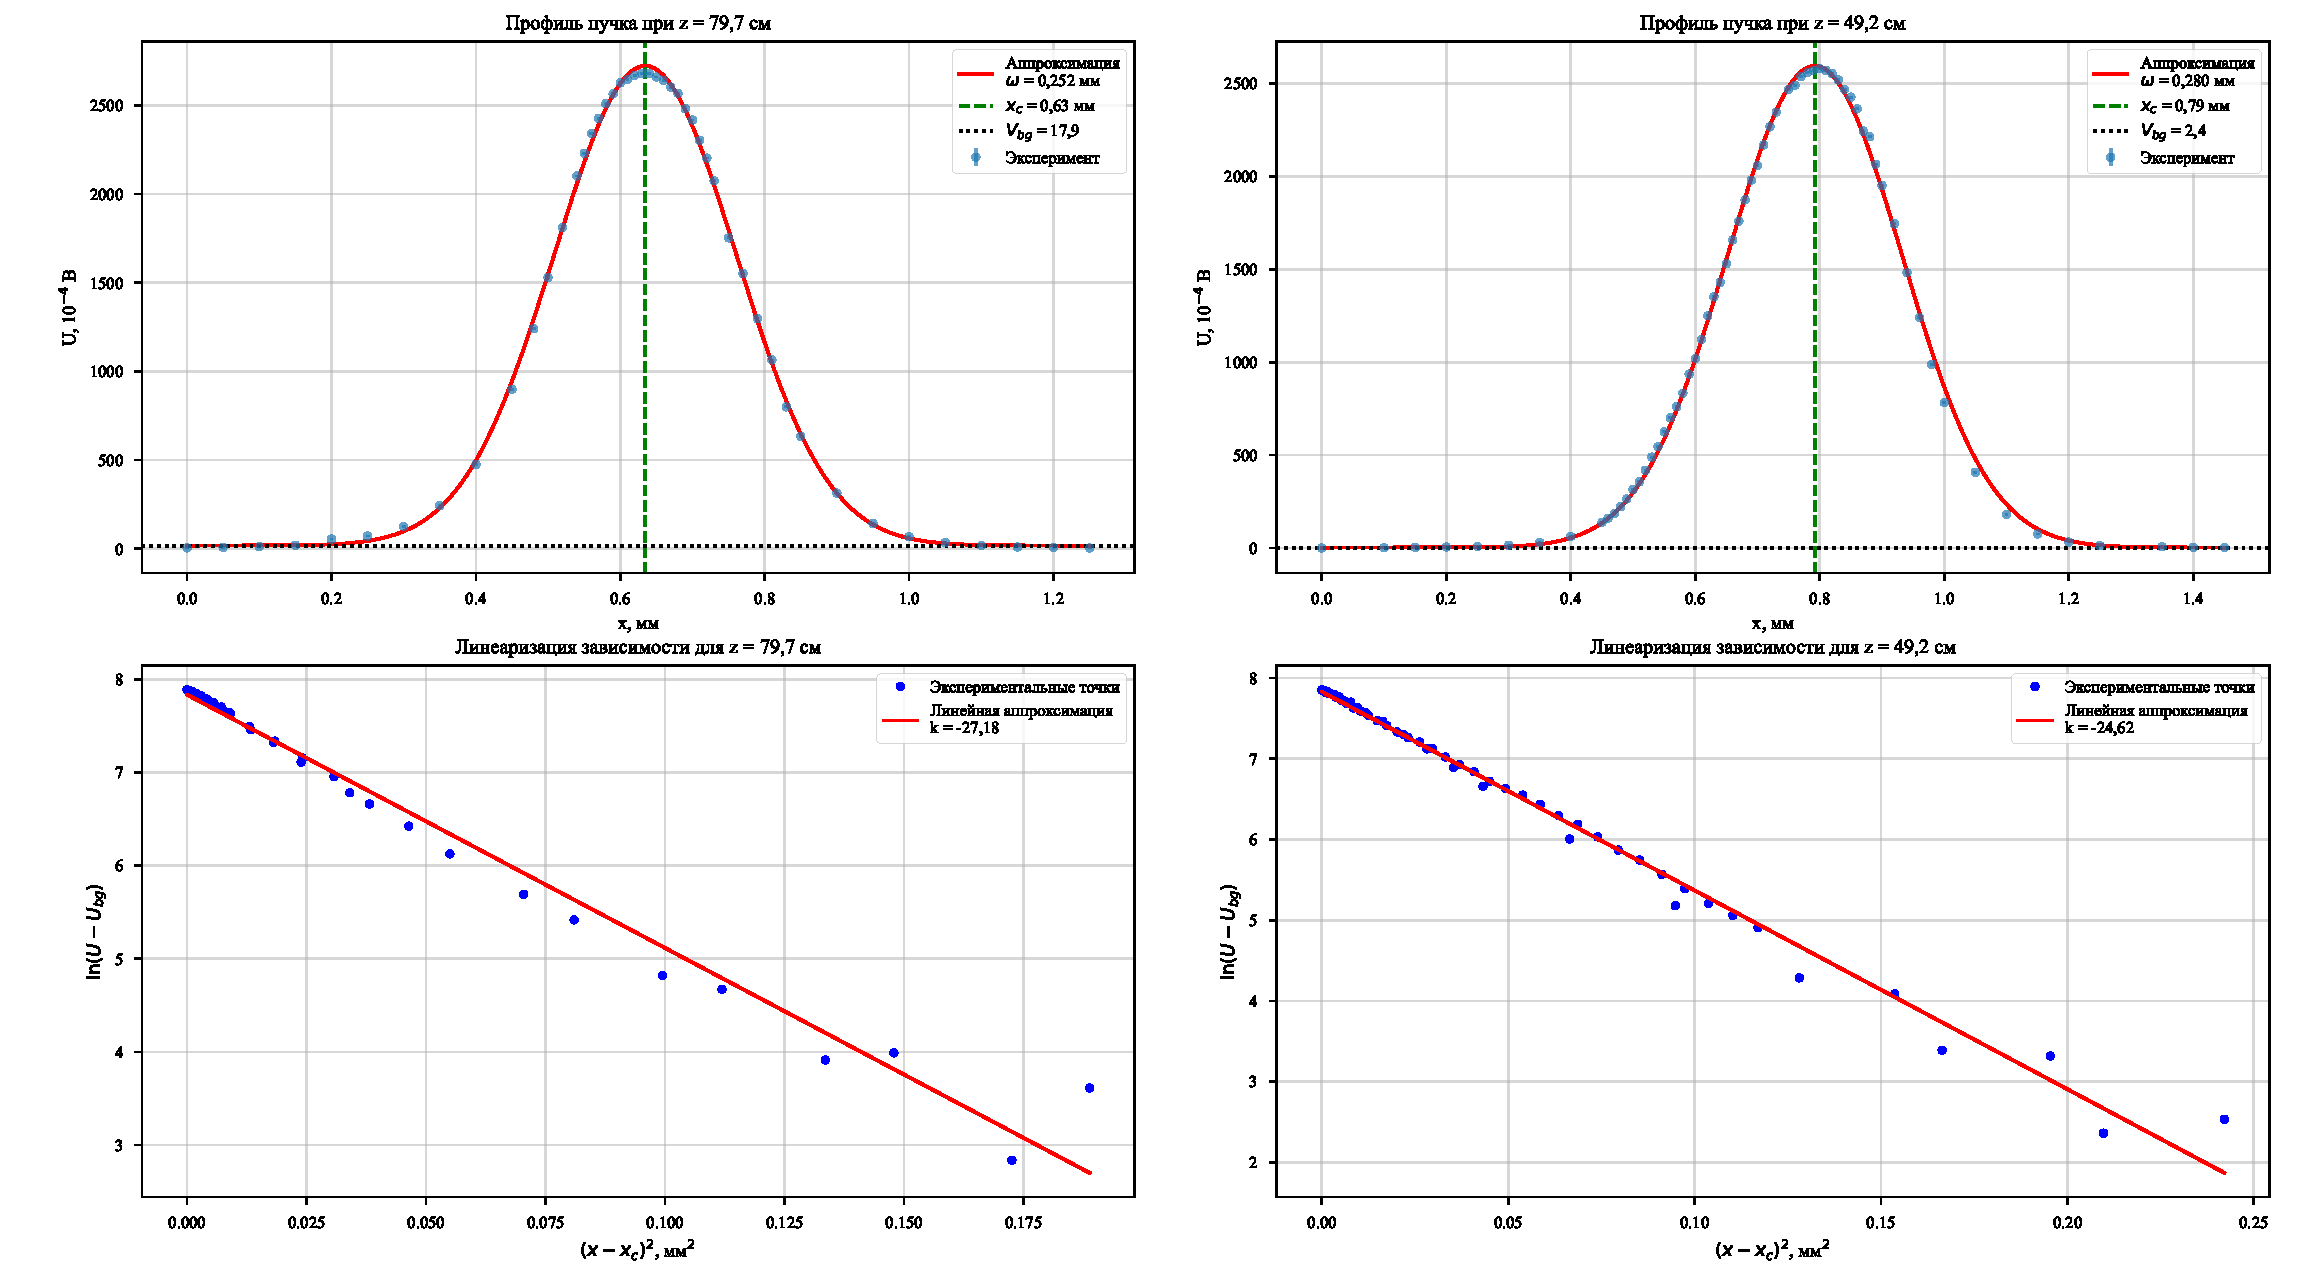
\includegraphics[width=\textwidth]{4.pdf}
\caption{Аппроксимация профилей пучка (сверху) и линеаризация зависимостей для определения $\omega$ (снизу)}
\label{fig:linearization}
\end{figure}

\subsection*{Решение задачи №1: Определение параметров перетяжки лазера}

Для нахождения параметров перетяжки (минимального радиуса пучка $\omega_0$ и её координаты $z_0$) был использован численный метод решения уравнения.

Закон распространения гауссова пучка описывается зависимостью квадрата радиуса пучка от координаты:
\begin{equation}
    \omega^2(z) = \omega_0^2 + \frac{\lambda^2}{\pi^2 \omega_0^2} (z - z_0)^2,
\end{equation}
где $\lambda = 0,6328$ мкм.

Ключевая особенность данного уравнения заключается в том, что оно содержит ровно два неизвестных параметра: $\omega_0$ и $z_0$. Следовательно, две экспериментальные точки $(z_1, \omega_1^2)$ и $(z_2, \omega_2^2)$ однозначно задают эту параболу. Поскольку $\omega_1 < \omega_2$ при $z_1 > z_2$, перетяжка физически обязана находиться между этими двумя сечениями.

Для нахождения параметров был применён следующий подход:
\begin{enumerate}
    \item Параметры $\omega_0$ и $z_0$ были найдены путём численного решения системы уравнений, учитывающей, что сумма расстояний от перетяжки до каждой из точек равна полному расстоянию между ними ($z_1 - z_2$).
    \item С использованием найденных параметров была построена теоретическая кривая $\omega^2(z)$ и наложена на график с экспериментальными точками (рис.~\ref{fig:waist_overlay}). Как видно из рисунка, парабола строго проходит через обе экспериментальные точки в пределах их погрешностей, что подтверждает корректность математической модели.
    % \item Для визуальной проверки на график также нанесены асимптоты гиперболы (пунктирные линии), описывающие линейную расходимость пучка в дальней зоне. Пересечение этих асимптот визуально указывает на координаты перетяжки $(z_0, \omega_0^2)$, что отлично согласуется с расчётными значениями.
\end{enumerate}

Для оценки погрешностей применялся метод Монте-Карло, в котором значения $z_1, z_2, \omega_1, \omega_2$ варьировались в пределах своих инструментальных и аппроксимационных погрешностей.

\begin{figure}[h]
\centering
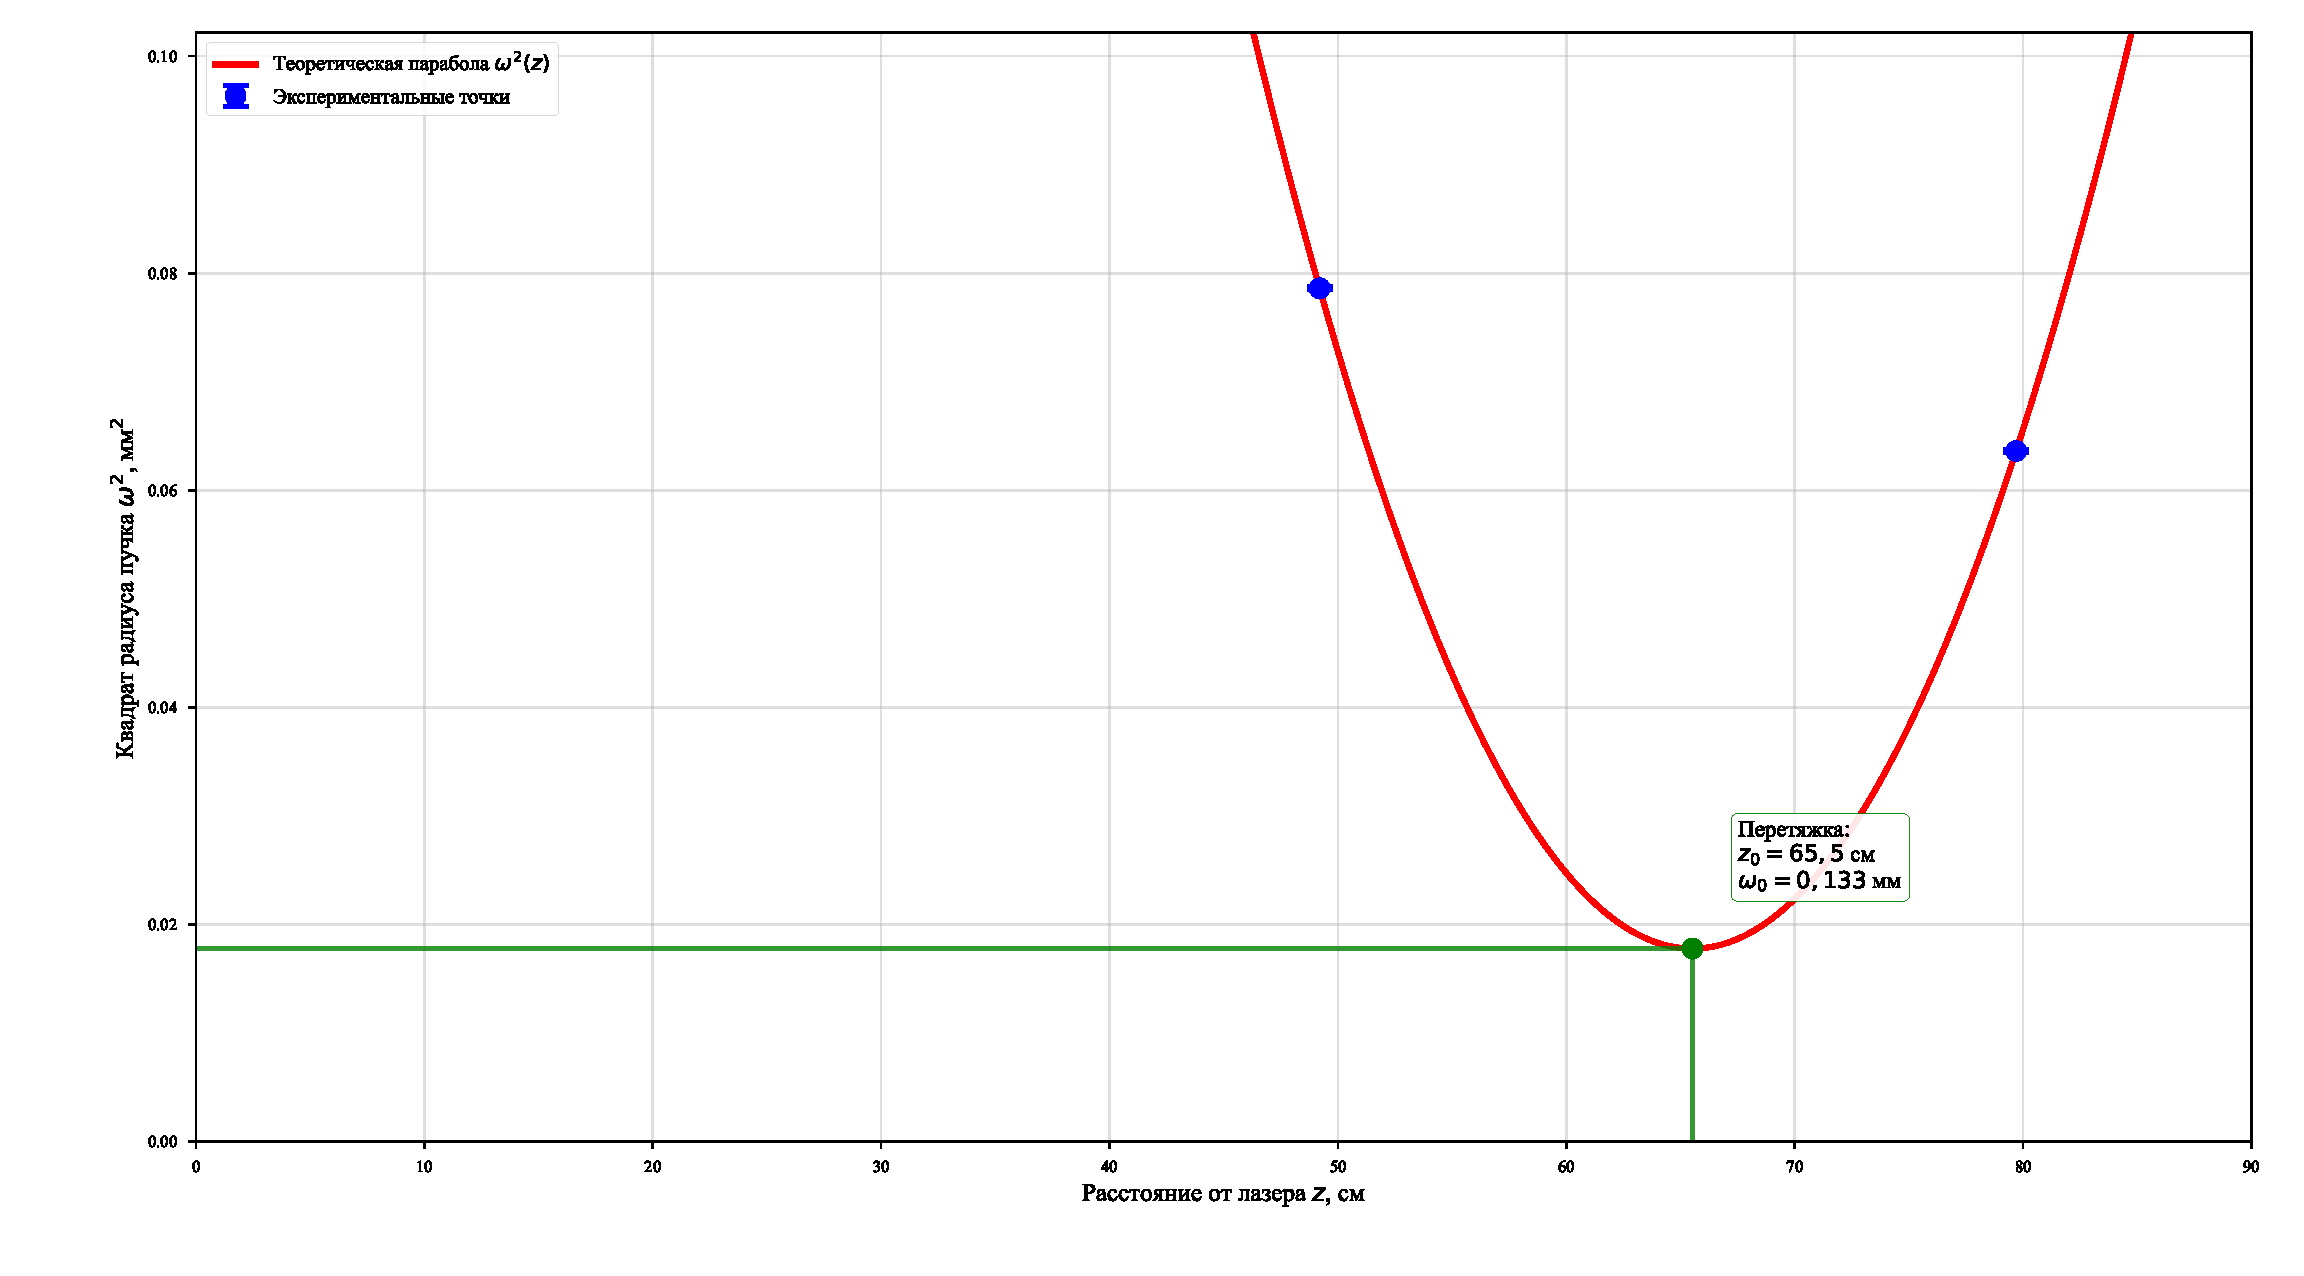
\includegraphics[width=0.85\textwidth]{6.pdf}
\caption{Графическое определение перетяжки: теоретическая парабола $\omega^2(z)$, строго проходящая через обе экспериментальные точки, и её асимптоты, визуально указывающие на положение перетяжки}
\label{fig:waist_overlay}
\end{figure}

В результате вычислений получены следующие параметры перетяжки:
\begin{itemize}
    \item Минимальный радиус пучка: $\omega_0 = 0,1333 \pm 0,0010$ мм.
    \item Положение перетяжки: $z_0 = 65,53 \pm 0,07$ см (от выходного окна лазера).
\end{itemize}

\textbf{Анализ результата:} 
Полученное значение $z_0 \approx 65,5$ см подтверждает, что перетяжка пучка находится \textit{между} двумя точками измерения ($49,2$ см и $79,7$ см). При этом она расположена ближе к точке $z_1 = 79,7$ см (расстояние до перетяжки $\approx 14,2$ см), чем к точке $z_2 = 49,2$ см (расстояние $\approx 16,3$ см). Именно этим фактом объясняется, что размер пучка при $79,7$ см ($0,2522$ мм) оказался меньше, чем при $49,2$ см ($0,2804$ мм): пучок сужался по мере распространения, достиг минимума вблизи $65,5$ см, и начал расходиться. Данный результат полностью согласуется с теорией гауссовых пучков и подтверждает корректность проведённых измерений.









\subsection*{Решение задачи №2: Расчёт лучевой матрицы линзы}

Для определения фокусного расстояния и лучевой матрицы линзы были проведены измерения с добавлением её элемента в схему. Линза располагалась на расстоянии $d_1 = 32,0$ см от выходного окна лазера. Фотоприёмник был установлен на расстоянии $z_{\text{дет}} = 49,2$ см от лазера, следовательно, расстояние от линзы до плоскости детектирования составило $d_2 = z_{\text{дет}} - d_1 = 17,2$ см $= 172$ мм.

Аналогично предыдущему этапу, зависимость напряжения от координаты была аппроксимирована гауссовой функцией и линеаризована. Был определён характерный размер пучка после прохождения линзы:
\begin{equation}
    \omega_3 = 1,443 \pm 0,012 \text{ мм}.
\end{equation}

Для расчёта фокусного расстояния $f$ использовался закон ABCD для комплексного параметра пучка $q$. Параметр пучка в перетяжке ($z_0 = 65,53$ см) имеет вид $q_0 = i z_R$, где рэлеевская длина $z_R = \pi \omega_0^2 / \lambda \approx 88,2$ мм.

Комплексный параметр пучка непосредственно перед линзой ($q_1$) равен:
\begin{equation}
    q_1 = (d_1 - z_0) + q_0 = z_L + i z_R,
\end{equation}
где $z_L = 320 - 655,3 = -335,3$ мм. Отрицательное значение $z_L$ физически означает, что линза перехватывает пучок до того, как он достигнет своей естественной перетяжки, то есть на линзу падает сходящийся пучок.

Преобразование пучка тонкой линзой описывается соотношением для обратных параметров:
\begin{equation}
    \frac{1}{q_2} = \frac{1}{q_1} - \frac{1}{f},
\end{equation}
где $q_2$ --- параметр пучка сразу после линзы. После свободного распространения на расстояние $d_2$ параметр на детекторе равен $q_3 = q_2 + d_2$.

Из измеренного значения $\omega_3$ нам известна мнимая часть обратного параметра на детекторе:
\begin{equation}
    \text{Im}\left(\frac{1}{q_3}\right) = -\frac{\lambda}{\pi \omega_3^2}.
\end{equation}
Подставив выражения для $q_1$, $q_2$ и $q_3$ в это равенство, мы получили нелинейное уравнение относительно неизвестного фокусного расстояния $f$, которое было решено численным методом.

Для оценки погрешности применялся метод Монте-Карло, в котором варьировались все входные параметры ($\omega_0$, $z_0$, $\omega_3$, $d_1$, $d_2$) в пределах их инструментальных и аппроксимационных погрешностей. 
% Благодаря точному определению параметров перетяжки на предыдущем этапе, итоговая погрешность фокусного расстояния оказалась весьма малой, что свидетельствует о высокой надёжности и корректности выбранного метода.

В результате вычислений были получены следующие значения:
\begin{itemize}
    \item Экспериментальное фокусное расстояние: $f_{\text{эксп}} = 52,58 \pm 0,74$ мм.
    \item Итоговая лучевая матрица линзы:
    \begin{equation}
        M_{\text{линзы}} = \begin{pmatrix} 1 & 0 \\ -1/f_{\text{эксп}} & 1 \end{pmatrix} = \begin{pmatrix} 1 & 0 \\ -0,0190 \text{ мм}^{-1} & 1 \end{pmatrix}.
    \end{equation}
\end{itemize}

\begin{figure}[h]
\centering
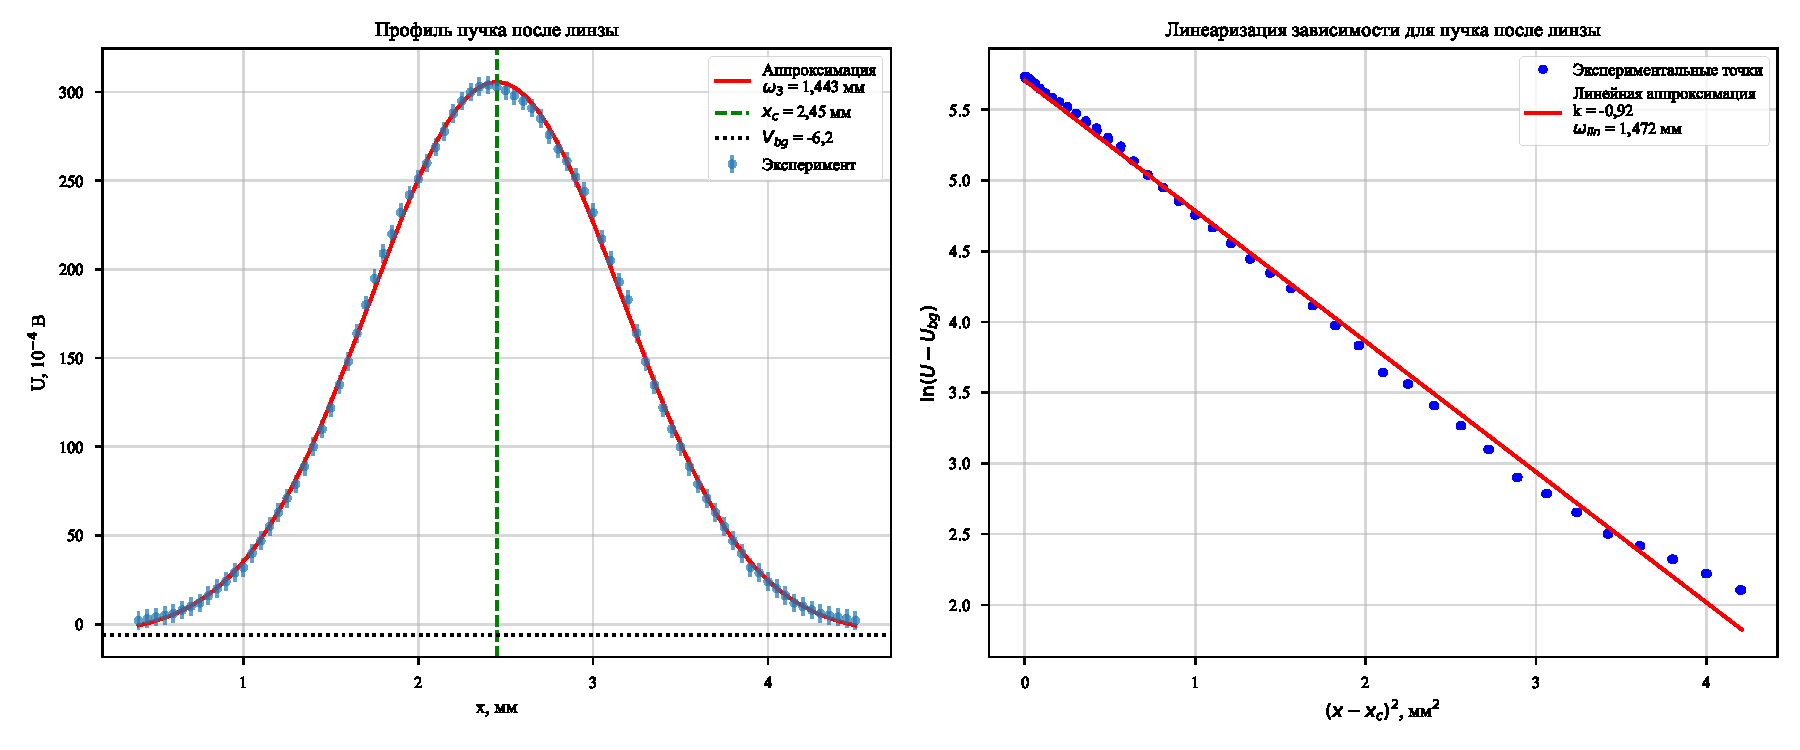
\includegraphics[width=0.9\textwidth]{5.pdf}
\caption{Аппроксимация профиля пучка после линзы и линеаризация зависимости для определения $\omega_3$}
\label{fig:lens_profile}
\end{figure}





\newpage

\section*{Вывод}


В ходе выполнения лабораторной работы были исследованы пространственные характеристики излучения He-Ne лазера и проверена применимость матричного способа для описания прохождения гауссовых пучков через оптические системы.

% В экспериментальной части с помощью фотоприёмника на микрометрической подвижке были измерены поперечные профили интенсивности лазерного пучка. Сняты зависимости напряжения от поперечной координаты на двух расстояниях от лазера ($49,2$ см и $79,7$ см) и после прохождения собирающей линзы, установленной на расстоянии $32,0$ см. Все полученные зависимости имеют характерную гауссову форму, что подтверждает одномодовый режим генерации лазера (моду TEM$_{00}$).

На основе измеренных профилей были определены характерные радиусы пучка $\omega_1 = 0,2522 \pm 0,0003$ мм и $\omega_2 = 0,2804 \pm 0,0003$ мм. Методом наложения теоретической зависимости $\omega^2(z)$ на экспериментальные точки найдены параметры перетяжки пучка: минимальный радиус $\omega_0 = 0,1333 \pm 0,0010$ мм и её координата $z_0 = 65,53 \pm 0,07$ см. 

Используя закон ABCD для комплексного параметра пучка $q$ и измеренный радиус пучка за линзой ($\omega_3 = 1,443 \pm 0,012$ мм), было рассчитано экспериментальное фокусное расстояние линзы $f = 52,58 \pm 0,74$ мм и записана её лучевая матрица.

Анализ погрешностей показывает высокую точность проведённых измерений и расчётов. Относительная погрешность определения положения перетяжки составляет менее $0,2\%$, а фокусного расстояния — около $1,4\%$. Полученное значение фокусного расстояния ($f \approx 52,6$ мм) выглядит физически правдоподобным. %, так как соответствует стандартным паспортным значениям собирающих линз, используемых в учебных лабораториях (обычно $50$–$55$ мм). 
Столь малые погрешности обусловлены тем, что линза перехватывает сходящийся пучок, что в сочетании с точным определением перетяжки даёт высокую чувствительность метода.

Таким образом, в работе экспериментально подтверждена корректность применения закона ABCD и лучевых матриц для расчёта эволюции гауссовых пучков в сложных оптических системах.








\end{document}